\documentclass[border=10pt]{standalone}
\usepackage{verbatim}
\usepackage{pgfplots}
\pgfplotsset{compat=1.14}

% stars_count = 512;
% max_time = 2.5
% steps = {0.1, 0.1 / 8, 0.1 / (8 * 8), 0.1 / (8 * 8 * 8), 0.1 / (8 * 8 * 8 * 8), 0.1 / (8 * 8 * 8 * 8 * 8)};

\begin{document}

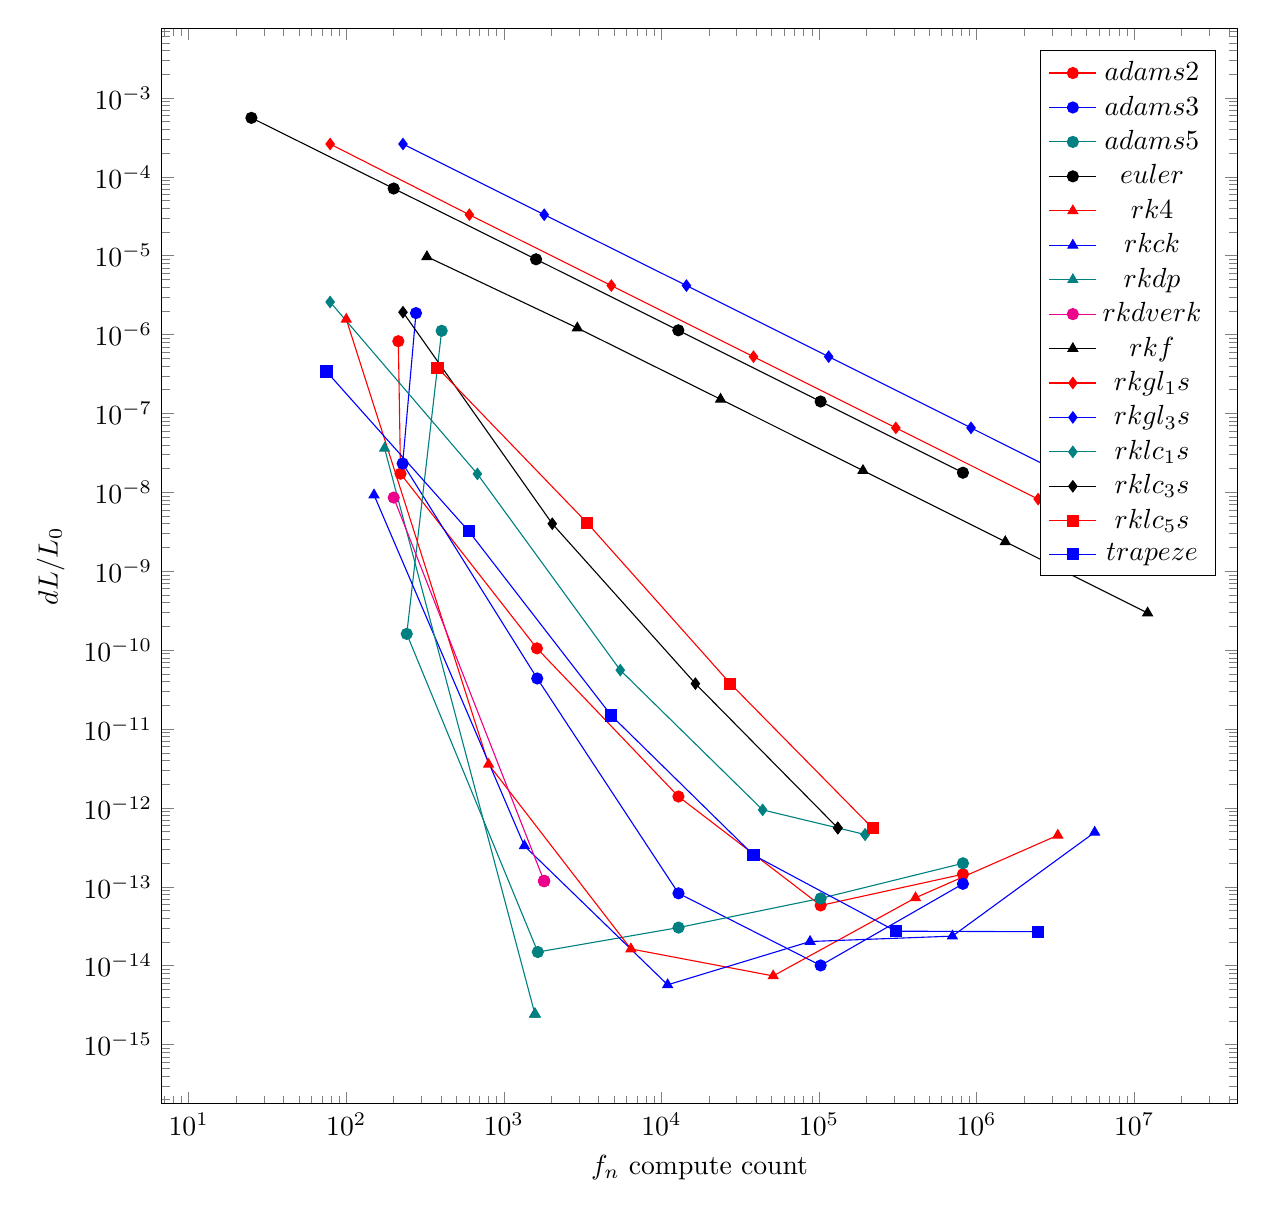
\begin{tikzpicture}
\begin{loglogaxis}[
    height=6in,
    width=6in,
    xlabel=$f_n$ compute count,
    ylabel=$dL/L_0$
]
\addplot [red,mark=*,solid] coordinates { (214, 8.252e-07) (221, 1.725e-08) (1622, 1.054e-10) (1.282e+04, 1.395e-12) (1.024e+05, 5.805e-14) (8.192e+05, 1.444e-13) };
\addplot [blue,mark=*,solid] coordinates { (277, 1.874e-06) (228, 2.327e-08) (1629, 4.374e-11) (1.283e+04, 8.268e-14) (1.024e+05, 1.007e-14) (8.192e+05, 1.091e-13) };
\addplot [teal,mark=*,solid] coordinates { (403, 1.117e-06) (242, 1.607e-10) (1643, 1.49e-14) (1.284e+04, 3.041e-14) (1.024e+05, 7.129e-14) (8.192e+05, 1.986e-13) };
\addplot [black,mark=*,solid] coordinates { (25, 0.0005593) (200, 7.107e-05) (1601, 9.009e-06) (1.28e+04, 1.134e-06) (1.024e+05, 1.419e-07) (8.192e+05, 1.775e-08) };
\addplot [red,mark=triangle*,solid] coordinates { (100, 1.562e-06) (800, 3.567e-12) (6404, 1.63e-14) (5.12e+04, 7.418e-15) (4.096e+05, 7.258e-14) (3.277e+06, 4.503e-13) };
\addplot [blue,mark=triangle*,solid] coordinates { (150, 9.265e-09) (1350, 3.305e-13) (1.095e+04, 5.724e-15) (8.775e+04, 2.025e-14) (7.022e+05, 2.37e-14) (5.617e+06, 4.907e-13) };
\addplot [teal,mark=triangle*,solid] coordinates { (175, 3.617e-08) (1575, 2.436e-15) (1575, 2.436e-15) (1575, 2.436e-15) (1575, 2.436e-15) (1575, 2.436e-15) };
\addplot [magenta,mark=*,solid] coordinates { (200, 8.583e-09) (1800, 1.184e-13) (1800, 1.184e-13) (1800, 1.184e-13) (1800, 1.184e-13) (1800, 1.184e-13) };
\addplot [black,mark=triangle*,solid] coordinates { (325, 9.718e-06) (2925, 1.214e-06) (2.372e+04, 1.515e-07) (1.901e+05, 1.893e-08) (1.521e+06, 2.366e-09) (1.217e+07, 2.958e-10) };
\addplot [red,mark=diamond*,solid] coordinates { (79, 0.0002606) (604, 3.309e-05) (4807, 4.186e-06) (3.841e+04, 5.254e-07) (3.072e+05, 6.572e-08) (2.458e+06, 8.216e-09) };
\addplot [blue,mark=diamond*,solid] coordinates { (229, 0.0002607) (1804, 3.309e-05) (1.441e+04, 4.186e-06) (1.152e+05, 5.254e-07) (9.216e+05, 6.572e-08) (7.373e+06, 8.216e-09) };
\addplot [teal,mark=diamond*,solid] coordinates { (79, 2.59e-06) (679, 1.714e-08) (5479, 5.581e-11) (4.388e+04, 9.441e-13) (1.961e+05, 4.6e-13) (1.961e+05, 4.6e-13) };
\addplot [black,mark=diamond*,solid] coordinates { (229, 1.924e-06) (2029, 4.006e-09) (1.643e+04, 3.762e-11) (1.316e+05, 5.563e-13) (1.316e+05, 5.563e-13) (1.316e+05, 5.563e-13) };
\addplot [red,mark=square*,solid] coordinates { (379, 3.804e-07) (3379, 4.098e-09) (2.738e+04, 3.762e-11) (2.194e+05, 5.504e-13) (2.194e+05, 5.504e-13) (2.194e+05, 5.504e-13) };
\addplot [blue,mark=square*,solid] coordinates { (75, 3.398e-07) (600, 3.205e-09) (4803, 1.486e-11) (3.84e+04, 2.525e-13) (3.072e+05, 2.738e-14) (2.458e+06, 2.696e-14) };
\legend{$adams2$,$adams3$,$adams5$,$euler$,$rk4$,$rkck$,$rkdp$,$rkdverk$,$rkf$,$rkgl_1s$,$rkgl_3s$,$rklc_1s$,$rklc_3s$,$rklc_5s$,$trapeze$};
\end{loglogaxis}
\end{tikzpicture}

\end{document}
